\documentclass{article}
\usepackage[english]{babel} %para a hifena��o entender Portugu�s
\usepackage[utf8]{inputenc} %para o pdflatex entender caracteres acentuados
\usepackage[T1]{fontenc} % para copy-paste do pdf entender caracteres acentuados
\usepackage{lmodern} % um fonte melhor para caracteres acentuados?
\begin{document}
  
\title{Cloud Computing}
\author{Paulo S. Abreu}
\date{}
 
 
\section{1. Basic underlying concepts.}
 
At a high - and overly simplistic - level, cloud services can be described as:
Consumer and business products, services, and solutions delivered and consumed in real time over a network (most often, the Internet). [5]
Cloud services can be defined more formally through a checklist of key attributes, which apply to all types of cloud services [5]:
Shared, standard service (built for multitenancy, among or within enterprises).
Solution packaged (a "turnkey" offering, pre-integrates required resources).
Self-service (provisioning and management, typically via a Web portal).
Elastic resource scaling (dynamic, rapid, and fine-grained).
Elastic, use-based pricing (supported by service metering).
Ubiquitous (authorized) network access (typically accessible via the Internet).
Standard User Interface technologies (browsers, and underlying technologies)
Published service interface/API (web services, other common Internet APIs - Application Programming Interfaces).
There are two types of deployment models for cloud services: public and private.

Public cloud services: Shared among unrelated enterprises and consumers, open to a largely unrestricted universe of potential users, designed for a market, not a single enterprise.
Private cloud services: Shared within a single enterprise or extended enterprise, with restrictions on access and level of resource dedication, defined/controlled by the enterprise, and beyond control available in public cloud offerings.

Under these attributes many types of services can be categorized as "cloud enabled". According to [5] "Toyota could claim that it is fundamentally the first real cloud provider by today's terms". (Note: there are many pages describing Toyota's case study in the article that are not worth repeating here).

However, for the remaining of this text, the term "cloud" will be restricted to computing services.

 

\section{2. Cloud computing is a type of cloud service.}

Hence, a definition of cloud computing would be:

Cloud computing is a method of providing a set of shared computing resources that includes applications, computing, storage, networking, development, and deployment platforms as well as business processes. Cloud computing turns traditional siloed computing assets into shared pools of resources that are based on an underlying Internet foundation. [1]
Cloud computing abides to the same eight attributes described above for generic cloud services and can also be deployed as a public or a private model. 

 

\section{3. The basics of IaaS, PaaS and SaaS.}

Cloud computing has been further broken down into categories depending on the allocation of IT resources. These categories are called IaaS, PaaS and SaaS (definitions for these terms are furhter down the text).

A simplified model on how IT resources allocation are distributed among these three categories and who owns the responsibility in each one of them is depicted below (adapted from [4]):

   Cloud Computing
 
 "In-house" enterprise IT
 Collocation
 IaaS
 PaaS
 SaaS
 
Data / Content Customer
 Customer
 Customer
 Customer
 Customer
 
Business Applications Software Customer
 Customer
 Customer
 Customer
 Service Provider
 
Database Management Customer
 Customer
 Customer
 Service Provider
 Service Provider
 
Middleware / Runtime Environment Customer
 Customer
 Customer
 Service Provider
 Service Provider
 
Operating System Customer
 Customer
 Service Provider
 Service Provider
 Service Provider
 
Servers / Virtualization Customer
 Customer
 Service Provider
 Service Provider
 Service Provider
 
Storage Customer
 Customer
 Service Provider
 Service Provider
 Service Provider
 
Facilities Customer
 Service Provider
 Service Provider
 Service Provider
 Service Provider
 


 

The terms IaaS, PaaS and SaaS are defined as:
\begin{itemize}
\item IaaS - Infrastructure as a Service: the delivery of hardware, storage, networking, data center space, and various utility software elements on request. IaaS is the fundamental element used by other cloud models. IaaS delivers various kinds of infrastructures, but when referring to computing services, it relates to delivering, at a minimum, Virtual Machines (VMs) as a service. Major features of IaaS are the freedom and the requirement that users are responsible for managing the VMs and everything above them. [2]
\item PaaS - Platform as a Service: a mechanism for combining IaaS with an abstracted set of middleware services, software development, and deployment tools that allow the organization to have a consistent way to create and deploy applications on a cloud or on-premises environment. A PaaS environment supports coordination between the developer and the operations organization. A PaaS offers a consistent set of programming and middleware services that ensure developers have a well-tested and well-integrated way to create applications in a cloud environment. A PaaS requires an infrastructure service. [1]
\item SaaS - Software as a Service: A business application created and hosted by a provider in a multi-tenant (shared) model. The SaaS application sits on top of both a PaaS and foundational IaaS. In fact, a SaaS environment can be built directly on an IaaS platform. Typically these underlying services aren�t visible to end-users of a SaaS application. [1]
\end{itemize}

\section{4. A more elaborate view on IaaS, PaaS, SaaS, public, private and hybrid clouds.}

IaaS:

Both public and private versions of IaaS exist (Note: compare these definitions with the ones provided in section 1 and you will see that they are very similar, these ones being a bit more practical from an IaaS perspective):

In the public IaaS (or public cloud), the user needs a simple sign-up mechanism to acquire resources. When users no longer need the resources, they simply de-provision them. [1]

In a private IaaS (or private cloud), the IT organization or an integrator creates an infrastructure designed to provide resources on demand (a managed pool of VMs) to internal users and sometimes partners. Some customers bring their own tools and software to create applications. [1, 3]

From a physical location perspective, IaaS can be furhter categorized as onsite or offsite, and can be managed by a third-party or by in-house staff. [5]

The next figure depicts the combination of all these subdivisions of IaaS:

\begin{figure}[ht!]
\centering
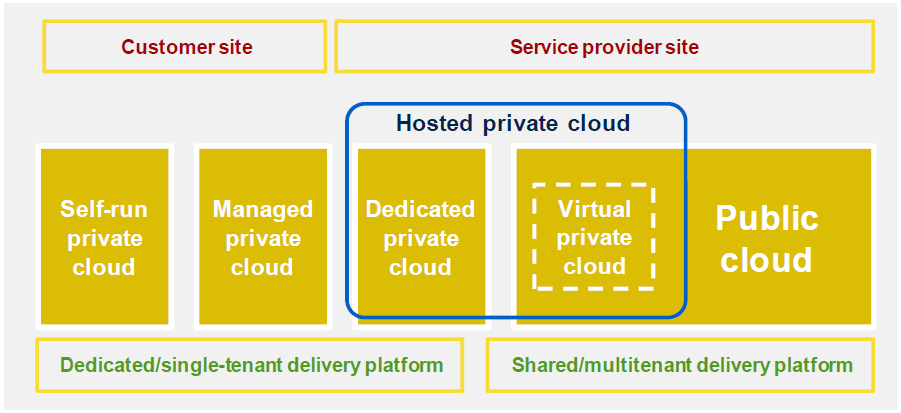
\includegraphics[width=90mm]{IDC_Cloud_services_deployment_methods.png}
\caption{IDC cloud deployment methods}
\end{figure}

Source: IDC [5]

In a private cloud that is managed by an in-house staff, "vendors (cloud Service Providers)" are equivalent to the IT departments/shared service departments within enterprises/groups. In this utilization model where standardized services are jointly used within the enterprise/group, business departments, offices, and employees are the "service users.".

Most organizations use a combination of private computing resources (data centers and private clouds) and public services. This is called a hybrid environment. A hybrid cloud combines private cloud computing services with public cloud computing services where one or several touch points exist between the environments. What does this mean? If a few developers in a company use a public cloud to prototype a new application that�s completely disconnected from the private cloud or the data center, the company doesn�t have a hybrid environment. [1]

 

PaaS:

If the the application infrastructure (middleware) functionality enriched with cloud characteristics is offered as a product (instead of a service), then the name CEAP (Cloud-Enabled Application Platform) is used, instead of PaaS. [3]
A Private PaaS is a service built by enterprise IT for use in enterprise IT projects of the same organization (but often a different IT center). The best practice of building a private PaaS for most IT organizations is by acquisition of a CEAP. (Gartner does not recommend building a private PaaS because it becomes a costly burden for most IT organizations). [3]
 

SaaS:

SaaS providers looking to retain control of their enabling technology without having to invent a new multitenant application server of their own use a CEAP (Cloud-Enabled Application Platform) product. [3]

 

\section{5. Glossary.}

API: Application Programming Interface.

BPaaS: Business Process as a Service.

DaaS: Database as a Service. Some providers uses this terminology for services associated to database storage and access on a cloud enviroment. Some of the features are: flexibility to expand the database, share information with other systems, easily provides remote access to authorized personel, others. (source: http://www.matrix.com.br/pt-BR/data-center/cloud)

SCI: Secure Cloud Interconnect. It is the naming Verizon gives for the interconnection between Verizon's Private IP Network to the Cloud Partner's Delivery Network.

TaaS: Testing as a Service. Some providers uses this terminology for services that are offered so the customers/users can test its applications and systems remotely, simulating its operational behavior (source: http://www.matrix.com.br/pt-BR/data-center/cloud)

XaaS: IT_component_X as a Service (related to xSP = x Service Provider).

 

References:

[1] Judith Hurwitz, Marcia Kaufman, Dr. Fern Halper, Cloud Services for Dummies, John Wiley & Sons, Inc, 2012.

[2] David Mitchell Smith, Daryl C. Plummer, Yefim V. Natis, Understand IaaS, PaaS and the Role of Middleware to Make the Most of Each, Gartner, ID:G00234828.

[3] Yefim V. Natis et al, Platform as a Service: Definition, Taxonomy and Vendor Landscape, 2013, Gartner, ID:G00247443.

[4] Melanie Posey et al, Directions 2013, IT Cloud Services at the Crossroads: How IaaS/PaaS/SaaS Business Models are Evolving, IDC, March 2013.

[5] David Tapper, Marianne Kolding, Industry Developments and Models. From Traditional to Cloud Services: A Market Framework, IDC, IDC#235783, July 2012.

Returns to wikirap home

Last modified at 6/24/2013 4:13 PM  by Belem, Fabio   
 
\end{document}  
    
 
  